%%%%%%%%%%%%%%%%%%%%%%%%%%%%%%%%%%%%%%%%%%%%%%%%%%%%%%%%%%%%%%%%%%%%%%%%%%%%%%%

To assess the recovery of SNR from template banks with NR waveforms or NR-PN 
hybrids as templates, we use the measures proposed in
Ref.~\cite{FittingFactorApostolatos,Sathyaprakash:1991mt,Balasubramanian:1995bm}. 
The gravitational waveform emitted during and driving a BBH coalescence is
denoted as $h(t)$, or simply $h$. The inner product between two 
waveforms $h_1$ and $h_2$ is
\begin{equation}\label{eq:overlap}
(h_1|h_2) \equiv 
4\int^{f_\mathrm{Ny}}_{f_\mathrm{min}}\dfrac{\tilde{h}_1(f)\tilde{h}_2^*(f)}{S_n(f)}\D f,
\end{equation}
where $S_n(f)$ is the one-sided power spectral density (PSD) of the detector
noise, which is assumed to be stationary and Gaussian with zero mean; 
$f_\mathrm{min}$ is the lower frequency cutoff for filtering; $f_\mathrm{Ny}$
is the Nyqyuist frequency corresponding to the waveform sampling rate; and 
$\tilde{h}(f)$ denotes the Fourier transform of $h(t)$.
% The noise PSD $S_n(f)$ is defined by
% \begin{equation}
%  \langle\tilde{n}(f)\tilde{n}^*(f')\rangle = \dfrac{1}{2}S_n(f)\delta(f-f'),
% \end{equation}
% where $\tilde{n}(f)$ is the Fourier transform of the detector noise $n(t)$, and
% $\langle\dots \rangle$ denotes an average over an ensemble of noise 
% realizations. 
In this paper, we take $S_n(|f|)$ to be the \textit{zero-detuning high power} 
noise curve for aLIGO, for both bank placement and overlap
calculations~\cite{aLIGONoiseCurve}; and set the lower frequency cutoff 
$f_\mathrm{min} =15$~Hz. The peak GW frequency for the lowest binary masses
that we consider, i.e. for $m_1+m_2\simeq 12M_\odot$, is $\sim 2.1$~kHz during
the ringdown phase. We sample the waveforms at $8192$~Hz, preserving the 
information content up to the Nyquist frequency $f_\mathrm{Ny}=4096$~Hz.
% The normalized overlap between the two waveforms,
% \begin{equation}
% (\hat{h}_1|\hat{h}_2) = \dfrac{(h_1|h_2)}{\sqrt{(h_1|h_1)(h_2|h_2)}},
% \end{equation}
% is also sensitive to a relative constant phase and time offset between $h_1$ 
% and $h_2$, $\phi_c$ and $t_c$, apart from the intrinsic mass parameters. These
A waveform, h, is normalized (made to be a unit vector) by 
$\hat{h} = h/\sqrt{h | h}$. In addition to being senstive to their 
intrinsic mass parameters, the inner product of two normalized waveforms is 
sensitive to phase and time shift differences between the two, $\phi_{c}$ and
$t_{c}$.  These two parameters ($\phi_c$ and $t_c$) can be analytically
maximized over to obtain the maximized overlap $\Olap$,
\begin{equation}\label{eq:maxnormolap}
\Olap(h_1,h_2) = 
\underset{\phi_c,t_c}{\mathrm{max}}\,\l(\hat{h}_1|\hat{h}_2(\phi_c,t_c)\r),
\end{equation}
which gives a measure of how ``close'' the two waveforms are in the waveform
manifold, disregarding differences in overall amplitude. The \textit{mismatch}
$\mathcal{M}$ between the two waveforms is then
\begin{equation}\label{eq:mismatch}
\mathcal{M}(h_1,h_2) = 1 - \Olap(h_1,h_2).
\end{equation}

Matched-filtering detection searches employ a discrete bank of modeled
waveforms as filters. The optimal signal-to-noise ratio (SNR) is obtained when
the detector strain $s(t)\equiv h^{\tr}(t) + n(t)$ is filtered with the 
\textit{true} waveform $h^{\tr}$ itself, i.e.
\begin{equation}
 \rho_{\mathrm{opt}} = \underset{\phi_c,t_c}{\mathrm{max}}\,\l(h^{\tr}|\hat{h}^{\tr}(\phi_c,t_c)\r) = \leftn h^{\tr}\rightn,
\end{equation}
where $\leftn h^{\tr}\rightn\equiv\sqrt{\left(h^{\tr},h^{\tr}\right)}$ is the
noise weighted norm of the waveform. With a discrete bank of filter templates, 
the SNR we recover
\begin{equation}\label{eq:realoptimalSNR}
 \rho\simeq \Olap(h^{\tr},h_b)\leftn h^{\tr}\rightn = \Olap(h^{\tr},h_b)\,\rho_{\mathrm{opt}},
\end{equation}
where $h_b$ is the filter template in the $b$ank (subscript $b$) that has the
highest overlap with the signal $h^{\tr}$.
The furthest distance to which GW signals can be detected is proportional to 
the matched-filter SNR that the search algorithm finds the signal with. 
Note that $0\leq\Olap(h^{\tr},h_b)\leq 1$, so the recovered SNR
$\rho\leq \rho_{\mathrm{opt}}$ (c.f. Eq.~(\ref{eq:realoptimalSNR})). 
For a BBH population uniformly distributed in spacial volume, the 
detection rate would decrease as $\Olap(h^{\tr},h_b)^3$. Searches that aim at
restricting the loss in the detection rate strictly below 
$10\%\,(\mathrm{or}\, 15\%)$, would require a bank of template waveforms that
have $\Olap$ above $0.965\,(\mathrm{or}\, 0.947)$ with \textit{any} incoming
signal~\citep{WaveformAccuracy2008,WaveformAccuracy2010}.


Any template bank has two sources for loss in SNR: 
(i) the discreteness of the bank grid in the physical parameter space of the 
BBHs, and, (ii) the disagreement between the actual GW signal $h^{\tr}$ and the 
modeled template waveforms used as filters. We de-coupled these to estimate
the SNR loss. Signal waveforms are denoted as $h^\tr_x$ in what follows, 
where the superscript $\tr$ indicates a $tr$ue signal, and the subscript
$x$ indicates the mass parameters of the corresponding binary. Template
waveforms are denoted as $h^\M_b$, where $\M$ denotes the waveform $m$odel, and
$b$ indicates that it is a member of the discrete \textit{b}ank.
% To put a bound on the 
% loss in SNR due to the first, we compute the \textit{minimal match} $\MM$ of 
% the bank,
% \begin{equation}
% \MM_{\mathcal{B}} = \underset{a}{\textrm{min}}\,\underset{g\, \in\, 
% \mathrm{bank}}{\textrm{max}}\,\Olap(h^{\M}_a,h^{\M}_g),
% \end{equation}
% \red{[Harald:  Define ``a'' in this equation and for use below]}
% which gives the highest fractional loss in SNR over the entire region of 
% physical parameters $\mathcal{B}$ that the bank covers. As both the signal 
% and the template 
% are modeled with the same approximant, $\MM$ measures the loss due to the 
% discreteness of the bank grid alone. The combined fractional SNR loss at any
% point $a$ in the parameter space can be measured by computing the 
% \textit{fitting factor} $\FF$ of the bank~\cite{FittingFactorApostolatos},
% \begin{equation}\label{eq:defFF}
% \FF_{\M}(a) = \underset{g\, \in\, 
% \mathrm{bank}}{\textrm{max}}\,\Olap(h^{\tr}_a,h^{\M}_g).
% \end{equation}
% which measures the same in a small neighborhood of $a$. A detection
% search that aims at strictly less than $10\%\,(15\%)$ loss in the observable  volume of the universe (module the effect of the cosmological redshift),
% requires a bank of template waveforms that has $\FF$ above $0.965\,
% (0.947)$~\citep{WaveformAccuracy2008,WaveformAccuracy2010,CompTemplates2009}
% over the entire parameter space.
\begin{figure}
 \centering
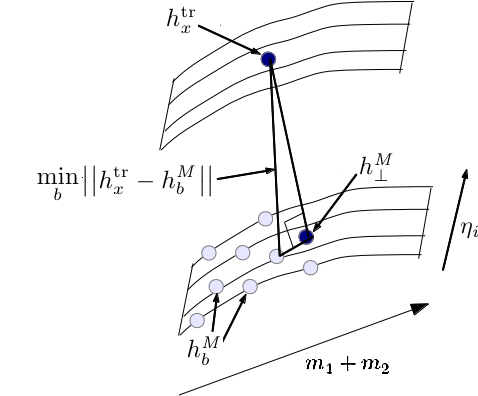
\includegraphics[width=\columnwidth]{Eff1v2.png}%\quad
\caption{We show the \textit{true} (upper) and the \textit{hybrid} (lower) 
waveform manifolds here, with the signal residing in the former, and a discrete
bank of templates placed along lines of constant mass-ratio in the latter. 
Both manifolds are embedded in the same space of all possible waveforms.
The true signal waveform is denoted as $h^{\tr}_x$, while the templates in the
bank are labelled $h^{\M}_b$. The hybrid waveform that matches the signal $H^{\tr}_x$
best is shown as $h^{\M}_\perp$. Also shown is the ``distance'' between
the signal and the hybrid template that has the highest overlap with it.
This figure is qualitatively similar to Fig.~3 of
Ref.~\cite{WaveformAccuracy2008}.}
\label{fig:EFFdiag1}
\end{figure}
% \begin{figure}
%  \centering
% 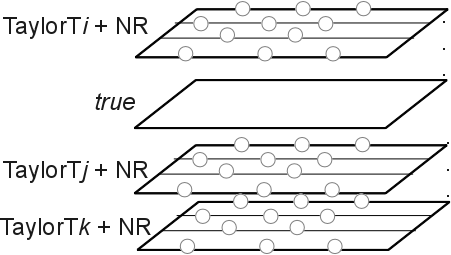
\includegraphics[width=0.8\columnwidth]{Eff2.png}%\quad
% \caption{We show the \textit{true} and the \textit{hybrid} waveform manifolds 
% relative to it. We assume that the hybrid waveform manifolds envelope 
% \textit{true} one, and so the shortest distance between a point on the true 
% manifold and any hybrid manifold would be lesser than the same between the two 
% mutually farthest hybrid manifolds; as for Eq.~(\ref{eq:hybridMMTn}).}
% \label{fig:EFFdiag2}
% \end{figure}
Fig.~\ref{fig:EFFdiag1} shows the signal $h^\tr_x$ in its manifold, and the
bank of templates $h^\M_b$ residing in the model waveform manifold, both being
embedded in the same space of all possible waveforms. The 
point $h^\M_\perp$ is the waveform which has the smallest mismatch
in the entire (continuous) model manifold with $h^\tr_x$, i.e.
$h^\M_\perp :\mathcal{M}(h^\tr_x,h^\M_\perp) = \underset{y}{\mn}\,\,\mathcal{M}(h^\tr_x,h^\M_y)$.
The fraction of the optimal SNR recovered at different points $x$ in the
binary mass space can be quantified by measuring the fitting factor $\FF$ of
the bank~\cite{FittingFactorApostolatos},
\begin{equation}\label{eq:ffmismatch}
 \FF(x) = 1 - \underset{b}{\mn}\,\,\mathcal{M}(h^\tr_x, h^\M_b).
\end{equation}
For two waveforms $h_1$ and $h_2$ close to each other in the
waveform manifold: $\leftn h_1\rightn \simeq\leftn h_2\rightn$, and mutually
aligned in phase and time such that the overlap between them is maximized, 
\begin{equation}
%  \begin{align}
  \leftn h_1 - h_2\rightn^2 \simeq 2\l( h_1 |h_1\r)\left(1 - \dfrac{\l( h_1 |h_2\r)}{\sqrt{\l( h_1 |h_1\r)}\sqrt{\l( h_1 |h_1\r)}}\right).
%  &= 2\leftn h_1\rightn^2 \Mis\left(h_1,h_2\right)
% \end{align}
\end{equation}
The mismatch can, hence, be written as 
(c.f. Eq.~(\ref{eq:mismatch}))
\begin{equation}
 \Mis\left(h_1,h_2\right) = \dfrac{1}{2\leftn h_1\rightn^2}\leftn h_1 - 
h_2\rightn^2.
\end{equation}
We note that this equation is an upper bound for Eq.~(25) of
Ref.~\cite{Cannon:2012gq}. 
From this relation, and treating the space embedding the true and model 
waveform manifolds as Euclidean at the scale of template separation, we
can separate out the effects of bank coarseness and template inaccuracies as
\begin{subequations}
\begin{align}
 \FF(x) &= 1 - \underset{b}{\mn}\dfrac{1}{2\leftn h^\tr_x\rightn^2}\leftn h^\tr_x - h^\M_b\rightn^2 ,\\
 &= 1 - \Gamma_\Hyb(x) - \Gamma_\bnk(x)\label{eq:FFGammas};
 %&= 1 - \underset{b}{\mn}\dfrac{1}{2\leftn h^\tr_x\rightn^2}\leftn h^\tr_x - h^\M_\perp\rightn^2 - \underset{b}{\mn}\dfrac{1}{2\leftn h^\tr_x\rightn^2}\leftn h^\M_\perp - h^\M_b\rightn^2
 \end{align}
\end{subequations}
where 
\begin{equation}
\Gamma_\Hyb(x) \equiv \dfrac{1}{2\leftn h^\tr_x\rightn^2}\leftn h^\tr_x - h^\M_\perp\rightn^2 = \mathcal{M}(h^\tr_x,h^\M_\perp) 
\end{equation}
is the SNR loss from model waveform errors out of the manifold of true signals;
and 
\begin{equation}\label{eq:GammaBank}
\Gamma_\bnk(x) \equiv \underset{b}{\mn}\dfrac{1}{2\leftn h^\tr_x\rightn^2}\leftn h^\M_\perp - h^\M_b\rightn^2 = \underset{b}{\mn}\,\,\mathcal{M}(h^\M_\perp,h^\M_b) 
\end{equation}
is the loss in SNR from the distant spacing of templates in the bank.
The decomposition in Eq.~(\ref{eq:FFGammas}) allows for the measurement of the 
two effects separately. 
% When we use the NR simulations as templates, $\Gamma_\Hyb \simeq 0$, but 
% hybridizing them with PN inspirals will introduce waveform errors. 
NR-PN hybrids have the inspiral portion of the waveform, from PN theory, 
joined to the available late-inspiral and merger portion from NR (as described
in Sec.~\ref{s2:NRpNhybridwaveforms}). Towards the late inspiral, the PN
waveforms accumulate phase errors, contaminating the
hybrids~\cite{MacDonald:2011ne,MacDonald:2012mp}. For each hybrid, we constrain
this effect using mismatches between hybrids constructed from the same NR 
simulation and different PN models, i.e.
\begin{equation}
 \Gamma_\Hyb(x) \leq \mathcal{M}(h^\tr_x,h^\Hyb_x) \lesssim \underset{(i,j)}{\mx}\,\,\mathcal{M}(h^{\M_i}_x,h^{\M_j}_x),
\end{equation}
where  $\M_i = $ TaylorT[1,2,3,4]+NR.
However, this is only possible for a few values of mass-ratio for which NR
simulations are available. We assume $\Gamma_\Hyb$ to be a slowly and smoothly 
varying quantity over the component-mass space at the scale of template grid
separation. At any arbitrary point $x$ in the mass space we approximate 
$\Gamma_\Hyb$ with its value for the ``closest'' template, i.e.
\begin{equation}\label{eq:GammaHybfinal}
 \Gamma_\Hyb(x) \leq \underset{(i,j)}{\mx}\,\,\mathcal{M}(h^{\M_i}_x,h^{\M_j}_x) \simeq \underset{(i,j)}{\mx}\,\,\mathcal{M}(h^{\M_i}_b,h^{\M_j}_b),
\end{equation}
where $h^\M_b$ is the hybrid template in the bank with the highest overlap with 
the signal at $x$. 
% Since NR waveforms have a limited number of 
% orbits, to obtain $\Gamma_\Hyb$ for hybrids with lower matching frequencies, 
% their NR portion is replaced with EOBNRv2 waveforms. As only the PN
% portion is changing in these comparisons, and the EOBNRv2 model was calibrated 
% against most of the NR simulations that we use here~\cite{BuonannoEOBv2Main}, 
% using EOBNRv2-PN hybrids gives the same measurements as using NR-PN hybrids for
% hybrid mismatches.

The other contribution to SNR loss comes from the discrete placement of 
templates in the mass space. In Fig.~\ref{fig:EFFdiag1}, this is shown in the
manifold of the template model. As NR waveforms (or hybrids) are available
for a few values of mass-ratio, we measure this in the manifold of EOBNRv2
waveforms. The EOBNRv2 model reproduces most of the NR simulations that
were consider here well~\cite{BuonannoEOBv2Main}, allowing for this 
approximation to hold. For the same reason, we expect $h^\EOB_x$ to be close to 
$h^\EOB_\perp$, with an injective mapping between the two. This allows us to 
approximate (c.f. Eq.~(\ref{eq:GammaBank}))
\begin{eqnarray}\label{eq:GammaBankEOB}
\label{eq:Gammabnkfinal}
 \Gamma_\bnk(x) &\simeq & \underset{b}{\mn}\,\,\mathcal{M}(h^\EOB_x,h^\EOB_b).
\end{eqnarray}

In Sec.~\ref{s1:NRonlybank}, we construct template banks that use purely-NR
templates, which have negligible waveform errors. The SNR recovery from such 
banks is characterized with
\begin{equation}\label{eq:NRFFGammas}
 \FF(x) = 1 - \Gamma_\bnk(x),
\end{equation}
where the SNR loss from bank coarseness is obtained using 
Eq.~(\ref{eq:Gammabnkfinal}). In 
Sec.~\ref{s1:NRpNhybridbank},~\ref{s1:futureNRpNhybridbank}, we construct 
template banks aimed at using NR-PN hybrid templates. Their SNR recovery is
characterized using Eq.~(\ref{eq:FFGammas}), where the additional contribution
from the hybrid waveform errors are obtained using Eq.~(\ref{eq:GammaHybfinal}).


% For the NR-PN hybrid template bank, as we do not know the \textit{true} 
% waveforms at arbitrary points in the signal parameter space (the component
% masses of the binary), we estimate the $\FF$ as follows. Let us
% parametrize the mass parameter space by $\eta$ and $M$, noting the bijective
% mapping
% $\eta =q/(1+q)^2$. 
% For any point in the mass space $(\eta,M)$, we re-write the $\FF$ as
% \begin{subequations}
% \begin{align}
%  \FF(\eta,M) &\equiv 1 - 
% \underset{\eta',M'}{\mn}\Mis\left(h^{\tr}(\eta,M),h^{\M}_g(\eta',M')\right) \\
%  %
%  \simeq & 1 - \dfrac{1}{2\leftn h\rightn^2}\,\, \underset{\eta',M'}{\mn} \leftn 
% h^{\tr}(\eta,M)-h^{\M}_g(\eta',M')\rightn^2 \label{eq:FFasnormsq} \\
%  \equiv & 1 - \dfrac{1}{2\leftn h\rightn^2}\,\E(\eta,M)
% \end{align}
% \end{subequations}
% where $\leftn h\rightn\equiv \leftn h^{\tr}(\eta,M)\rightn \simeq \leftn 
% h^{\M}_g(\eta',M')\rightn$, and $\E(\eta,M)\equiv \underset{\eta',M'}{\mn} \leftn 
% h^{\tr}(\eta,M)-h^{\M}_g(\eta',M')\rightn^2$. 
% %What we want to constrain, at each point $(\eta ,M)$ in the region of 
% %component mass space that our NR-PN-hybrid bank aims to cover is
% % \begin{multline}
% %  \underset{\eta_i,M_A}{\mn} \leftn h^{\tr}(\eta,M) - 
% % h^{\M}_g(\eta_i,M_A)\rightn^2 \notag\\
% %  = 2\rho\,(1-\FF_{\Hyb}(\eta,M)) \equiv \E(\eta,M),
% % \end{multline}
% %where $\rho$ in the expected matched-filter signal-to-noise-ratio (SNR) for the 
% %signal with source parameters $(\eta, M)$.
% As in Ref.~\cite{WaveformAccuracy2008,WaveformAccuracy2010}, we visualize the
% waveforms in their manifold in Fig.~\ref{fig:EFFdiag1}, where the top manifold
% is that of the \textit{true} waveforms, and the bottom is the model waveform 
% manifold; while the parallel lines are contours of constant mass-ratio with 
% total mass $M$ increasing from left to right (clockwise). The NR and the NR-PN
% hybrid bank grids are restricted to occupy these contours as NR simulations are 
% only available for a discrete set of mass-ratios, but can be rescaled to 
% different values of total mass. The quantity $\E$ is depicted in the figure as
% the ``distance'' between the \textit{true} signal and the \textit{closest}
% template in the bank of hybrid waveforms (squared). We drop a \red{[Word missing here?]} perpendicular 
% from the signal at $(\eta, M)$ in the \textit{true} manifold to the hybrid 
% waveform manifold at $(\eta_{\perp}'', M_{\perp}'')$, i.e.
% \begin{multline}
% (\eta_{\perp}'', M_{\perp}''):\,\leftn h^{\tr}(\eta,M) - h^{\M}(\eta_{\perp}'', M_{\perp}'')\rightn \notag\\
%  = \underset{\eta'',M''}{\mn} \leftn h^{\tr}(\eta,M) - h^{\M}(\eta'', 
% M'')\rightn.
% \end{multline}
% As waveforms are smooth functions of the masses, their manifolds are
% expected to be smooth and the mapping $T:(\eta,M)\rightarrow (\eta_{\perp}'', 
% M_{\perp}'')$ to be unique. Assuming both true and approximant waveform 
% manifolds are in a locally Euclidean space (over ``distances''
% at the scale of template separation) we can write $\E(\eta,M)$ as
% \begin{subequations}
% \begin{align}
%  \E(\eta,M) &= \underset{\eta'',M''}{\mn} \leftn h^{\tr}(\eta,M) - h^{\M}(\eta'', M'')\rightn^2 \notag\\
%  & + \underset{\eta',M'}{\mn} \leftn h^{\M}(\eta_{\perp}'', M_{\perp}'') - 
% h^{\M}_g(\eta', M')\rightn^2 \label{eq:MMaddQuad1}\\
%  &\equiv \Delta_1 + \Delta_2(\eta_{\perp}'', M_{\perp}''),
% \end{align}
% \end{subequations}
% where $\Delta_1 =\Delta_1(\eta,M) =\Delta_1\left(T^{-1}(\eta_{\perp}'', M_{\perp}'')\right)$ 
% and $\Delta_2(\eta_{\perp}'', M_{\perp}'')$ are 
% abbreviations for the first and second terms in Eq.~\ref{eq:MMaddQuad1}, 
% respectively. 
% 
% \red{[Harald:  The description here seems overly complicated.  Please reconsider whether all symbols introduced are really needed.  Also reconsider ordering to make the flow of ideas as smooth and uninterrupted as possible.  Specifically: (i) Is a symbol needed for the mapping $T$, or is it sufficient to define $\eta_\perp$ and $M_\perp$?  (ii) Do the symbols $\Delta_1$ and $\Delta_2$ need to have parameters attached to it inside parentheses?  If so, they are defined as functions, so define what the functions are.  I see $\Delta_1(...)$ used below {\em once} with different arguments.  If this is the only use, then it's easier to just spell out that one use, rather than to define a function (iii) if $\Delta_1$ needs to remain a function, be consistent with how you write it.  Either always with arguments or never.]}
% 
% The first of these
% \begin{equation}
%   \Delta_1(\eta,M)\leq \underset{M''}{\mn} \leftn h^{\tr}(\eta,M) - h^{\M}(\eta, M'')\rightn^2,
% \end{equation}
% where the RHS of this inequality is the quantity that we put a bound on to
% estimate the waveform errors for the NR-PN hybrids~\cite{MacDonald:2012mp}. 
% The hybridization of NR 
% simulations with different PN waveforms gives us different hybrids, all of which 
% reside in their own manifolds, as shown in Fig.~\ref{fig:EFFdiag2}. If we assume 
% that the \textit{true} manifold is enveloped between the different hybrid 
% manifolds, we can conservatively estimate
% \begin{equation}\label{eq:hybridMMTn}
%  \begin{split}
%   \Delta_1 & \leq \underset{M''}{\mn} \leftn h^{\tr}(\eta,M) - h^{\M}(\eta, M'')\rightn^2 \\
%   &\lesssim \underset{(i,j)}{\max}\, \underset{M''}{\mn} \leftn h^{\M_i}(\eta,M) - h^{\M_j}(\eta, M'')\rightn^2,
%  \end{split}
% \end{equation}
% \red{[Harald:  I don't think we ever did the minimization over $M''$ when computing PN-hybrid errors.]}
% \red{[Harald: The text presently discusses twice how PN-hybrid errors are determined, here and in Sec IIF.  It would be good to incorporate IIF into IIE.  However, spend an entire paragraph on how they are determined, they are too complicated to do in passing in a sentence or two.]}
% 
% 
% where $(\M_i,\M_j)$ are pairs of the same NR waveform hybridized with 
% different PN approximants. As we have NR simulations for restricted values of
% mass-ratio, estimation of $\Delta_1$ at arbitrary points in the component-mass
% space is difficult. Assuming $\Delta_1$ to be a slowly varying quantity over the 
% component-mass space at the scale of template grid separation, we approximate 
% $\Delta_1 (\eta_{\perp}'', M_{\perp}'')\simeq\Delta_1(\eta_{g_c},M_{g_c})$,
% where $(\eta_{g_c},M_{g_c})$ is the closest template grid point to 
% $(\eta_{\perp}'', M_{\perp}'')$, obtained by maximizing
% $\Olap(h^{\M}(\eta_{\perp}'', M_{\perp}''),h^{\M}(\eta_{g_c},M_{g_c}))$.
% Then, the fitting factor at a point $(\eta,M)$ in the true manifold, and at
% $(\eta_{\perp}'', M_{\perp}'')$ in the model waveform manifold becomes
% %\begin{equation}
% \begin{subequations}\label{eq:FFConstraint}
%  \begin{align}
% \FF(\eta,M) &\lesssim 1 - \underset{(i,j)}{\mx}\,\underset{M''}{\mn}\,\,  \mathcal{M}\left(h^{\M_i}(\eta_{g_c},M_{g_c}), h^{\M_j}(\eta_{g_c}, M'')\right) \label{eq:effdef1}\notag\\
%  &\,\, - \underset{\eta_i,M_A}{\mn}\mathcal{M}\left(h^{\M}(\eta_{\perp}'', M_{\perp}''),h^{\M}_g(\eta_i, M_A)\right)  \\
%  &\equiv 1 - \Gamma_{\Hyb}(\eta_{\perp}'', M_{\perp}'') - \Gamma_{\bnk}(\eta_{\perp}'', M_{\perp}'') \\
%  &= 1 - \Gamma_{\Hyb}\left(T(\eta, M)\right) - \Gamma_{\bnk}\left(T(\eta, M)\right) ,
%  \end{align}
% \end{subequations}
% %\end{equation}
% where $\Gamma_{\Hyb}$ and $\Gamma_{\bnk}$ are just the last two terms on the 
% RHS of Eq.~\ref{eq:effdef1}. To construct an effectual bank, therefore, we
% restrict $\Gamma_{\Hyb} + \Gamma_{\bnk}$ below $0.035\,(0.053)$ over the region
% the NR-only or the NR-PN hybrid bank is to cover, as discussed above.
% 
% 
% \red{[Harald: I didn't manage to follow the calculation in Sec IIE
%   within the time I spent on it.  Perhaps it would be clearer to
%   reorganize the argument to arrive quickly at
% \begin{equation}
% FF(\eta, M) \lesssim 1- \Gamma_{\rm Hyb} - \Gamma_{\rm bank},
% \end{equation}
% as a sum of terms orthogonal to the model manifold, and tangential to
% the model manifold.  After this equation has been obtained, consider
% each of the $\Gamma_{\rm bank/Hyb}$ separately with its own sequence
% of inequalities.]}
% 
% 
% 
% 
% % From Eq.~\ref{eq:FFasnormsq}
% % \begin{equation}
% %  \FF(\eta,M) = 1 - \dfrac{1}{2\leftn h\rightn^2}\,\, \underset{\eta',M'}{\mn}
% %\leftn h^{\tr}(\eta,M)-h^{\M}_g(\eta',M')\rightn^2,
% % \end{equation}
% % we need to find an upper bound on
% % $\leftn h^{\tr}(\eta,M)-h^{\M}_g(\eta',M')\rightn^2$, which we can constrain
% % over the component-mass region. Let 
% % \begin{equation}
% %  \epsilon_{\Hyb}(\eta,M) \equiv \leftn h^{\tr}(\eta,M)-h^{M}(\eta,M)\rightn^2,
% % \end{equation}
% % be the error norm for the Hybrid waveform ($\M = \Hyb$ here), and
% % \begin{equation}
% %  \epsilon_{\Hyb,\eta,\M}(\eta,M) \equiv \underset{\eta'',M''}{\mn}\leftn 
% % h^{\tr}(\eta,M)-h^{M}(\eta'',M'')\rightn^2
% % % \end{equation}
% % % is the waveform error norm margenalized over the subscripted mass parameters. 
% % % Also define $(\eta'_m,M'_m)$ as the parameter values on the model manifold
% % % \begin{multline}
% % %  (\eta'_m,M'_m): \leftn h^{\tr}(\eta,M) - h^{\M}(\eta'_m,M'_m)\rightn^2 = \\
% % %  \underset{\eta'',M''}{\mn}\leftn h^{\tr}(\eta,M) - 
% % h^{\M}(\eta'',M'')\rightn^2,
% % % \end{multline}
% % % at which the line drawn from the manifold of true waveforms starting at 
% % ($\eta,M$)
% % % is orthogonal to the $\M$ manifold (which is the manifold of Hybrid waveforms 
% % in
% % % our case). We can then write
% % % \begin{subequations}
% % %  \begin{align}
% % %   &\underset{\eta',M'}{\mn}\leftn h^{\tr}(\eta,M)-h^{\M}_g(\eta',M')\rightn^2 
% % \simeq \notag\\
% % %   &\quad\quad \leftn h^{\tr}(\eta,M) - h^{\M}(\eta'_m,M'_m)\rightn^2 +\notag\\
% % %   &\quad\quad\quad\quad\underset{\eta',M'}{\mn} \leftn h^{\M}(\eta'_m,M'_m) - 
% % h^{\M}_g(\eta',M')\rightn^2 \\
% % %   %
% % %   &= \epsilon_{\Hyb,\eta,\M}(\eta,M) + \epsilon_{\mm}(\eta'_m,M'_m) \\
% % %   %
% % %   &\leq \epsilon_{\Hyb,\M}(\eta,M) + 
% % \epsilon_{\mm}(\eta'_m,M'_m)\label{eq:mmtogridmm}
% % %  \end{align}
% % % \end{subequations}
% % % where $\epsilon_{\Hyb,\M}(\eta,M)$ is the hybrid waveform error minimized 
% % over 
% % only the total mass at the point ($\eta,M$) and $\epsilon_{\mm}(\eta'_m,M'_m)$ 
% % is the loss due to 
% % % discretization of the bank grid at the point ($\eta'_m,M'_m$). Now, if we 
% % term 
% % the
% % % maximum loss due to a discrete grid $\epsilon_g$ (and call it \textit{grid} 
% % maximal
% % % mismatch), i.e.
% % % \begin{align}
% % %  \epsilon_g &\equiv 
% % \underset{\eta'_m,M'_m}{\mx}\epsilon_{\mm}(\eta'_m,M'_m)\notag\\
% % %  &\equiv \underset{\eta'_m,M'_m}{\mx}\underset{\eta',M'}{\mn} \leftn 
% % h^{\M}(\eta'_m,M'_m) - h^{\M}_g(\eta',M')\rightn^2,
% % % \end{align}
% % % we have, from Eq.~\ref{eq:mmtogridmm},
% % % \begin{equation}
% % %  \underset{\eta',M'}{\mn}\leftn h^{\tr}(\eta,M)-h^{\M}_g(\eta',M')\rightn^2 
% % \leq  \epsilon_{\Hyb,\M}(\eta,M) + \epsilon_g.
% % % \end{equation}
% % % \textit{If we assume that $\epsilon_{\Hyb,\M}(\eta,M)$ is a slowly varying 
% % function of the 
% % % mass-parameters compared to the grid density}, 
% % % i.e. $\epsilon_{\Hyb,\M}(\eta,M)\simeq \epsilon_{\Hyb,\M}(\eta',M')$,
% % % where $(\eta',M')$ are the parameters values of the closest point on the grid 
% % to
% % % ($\eta,M$), we get
% % % \begin{subequations}
% % % \begin{align}\label{eq:Finmms}
% % %  \underset{\eta',M'}{\mn}\leftn h^{\tr}(\eta,M)-h^{\M}_g(\eta',M')\rightn^2 
% % \leq  \epsilon_{\Hyb,\M}(\eta',M') + \epsilon_g \\ \label{eq:FinFFs}
% % %  \Rightarrow \FF(\eta,M) \geq 1 - \dfrac{1}{2\leftn 
% % h\rightn^2}\,\,\left(\epsilon_{\Hyb,\M}(\eta',M') + \epsilon_g\right)
% % % \end{align}
% % % \end{subequations}
% % % If we construct a bank, with 
% % % \begin{equation}
% % % \boxed{ \dfrac{1}{2\leftn h\rightn^2}\,\,\left(\epsilon_{\Hyb,\M}(\eta',M') + 
% % \epsilon_g\right) \leq 0.035;\,\,\forall\,(\eta',M')\in\mathrm{bank}},
% % % \end{equation}
% % % it should restrict the detection rate loss to below $\sim 10\%$. In other 
% % words,
% % % the tolerances we have to construct the NR-PN hybrid bank is
% % % \begin{equation}
% % %  \boxed{\MM_{\Hyb,\M} + \MM_g \leq 0.035}
% % % \end{equation}
% % % where $\MM_{\Hyb,\M}\equiv \underset{\eta',M'}{\mx}\left(\dfrac{1}{2\leftn 
% % h\rightn^2}\epsilon_{\Hyb,\M}(\eta',M')\right)$ is the hybrid waveform 
% % mismatch, 
% % % minimized over total-mass for each point in the bank, and subsequently 
% % maximized
% % % over the entire bank; and $\MM_g\equiv\dfrac{1}{2\leftn 
% % h\rightn^2}\,\epsilon_g$
% % % is the discretization mismatch measured using the same model as signal and 
% % template.
% 
% %\red{\em Describe how we derive an error-bound on a PN-NR hybrid waveform.}
% 
% The largest source of error in hybrid gravitational waveforms is
% caused by the higher-order unknown terms in the PN component. These
% cause different PN approximants to diverge as the binary black holes approach
% merger. In order to ascertain what this error is, we compare many
% types of PN waveforms and find the maximum mismatch between hybrids
% which use different PN approximants, in this case, Taylor T1, T2, T3,
% and T4. We assume this to be close to the actual PN error, as discussed in 
% Sec.~\ref{s2:quantifyingerrors}.
% 
% More specifically, we take four hybrid waveforms $h_\text{Tn}$, where $n = [1,2,3,4]$, and find their mismatches as defined in Eq.~\ref{eq:mismatch}:
% \begin{equation}
% \mathcal{M}_\text{max}(\eta,M) = \underset{(i,j)}{\mx}\,\underset{M''}{\mn}\,\,  \mathcal{M}\left(h^{\mathrm{T}i}(\eta,M), h^{\mathrm{T}j}(\eta,M'')\right) 
% \end{equation}
% $\mathcal{M}_\text{max}$ is what we call the hybridization error.
% 
% Because NR waveforms have a limited number of orbits, to obtain results for hybrids with lower matching frequencies, we replace the NR part of the hybrids with EOBNRv2 waveforms as described in Sec.~\ref{s2:EOBwaveforms}. Since only the PN waveforms are changing in these hybrid comparisons, using EOB hybrids gives the same results as using NR hybrids.
